% Title page.
\title[Aula 06]{4. Distribuições e variações temporais das propriedades físicas}
\subtitle{(horizontais e verticais)}
\author[Filipe Fernandes]{Filipe P. A. Fernandes}
\institute[unimonte]{Centro Universitário Monte Serrat}
\date[Outubro 2013]{16 de Outubro 2013}

\logo{
\includegraphics[scale=0.15]{../common/university_logo.png}}

\begin{document}

% The title page frame.
\begin{frame}[plain]
  \titlepage
\end{frame}

\section*{Outline}
\begin{frame}
\tableofcontents
\end{frame}


\section{Considerações gerais}
\begin{frame}
  \frametitle{Considerações gerais}
  \begin{block}{}
    O oceano está mecanicamente e termicamente acoplado à atmosfera;

    As interações ar-mar são de vital importância para estudo de
    variações climáticas oceânicas (e terrestres);
  \end{block}
\end{frame}


\begin{frame}
  \frametitle{Considerações gerais}
  \begin{block}{}
    Um dos aspectos mais salientes sobre a distribuição de temperatura/salinidade nos oceanos é a sua estratificação.

    Exemplo: No equador a temperatura varia entre 25\textcelsius{} na
   superfície e 5\textcelsius em 1.000 m.  Porém, é necessário deslocar
   5.000 km para norte ou para sul para baixar para os mesmo 5\textcelsius.

   O gradiente vertical da temperatura é 5000 vezes superior ao gradiente
   horizontal.
  \end{block}
\end{frame}


\begin{frame}
\frametitle{Camadas}
  \begin{center}
    \includegraphics[scale=0.3]{../figures/camadas.png}
  \end{center}
\end{frame}


\section{Distribuições horizontais}
\begin{frame}
  \frametitle{Distribuição horizontal temperatura}
  \small{
  \begin{itemize}[<+-| alert@+>]
    \item A distribuição da temperatura à superfície no oceano é
          aproximadamente zonal;
    \item As isolinhas de temperatura seguem aproximadamente os paralelos de
          latitude;
    \item Perto da costa oeste as isotermas tendem a direção norte-sul;
    \item Na margem leste, entretanto, ocorrem baixas temperaturas junto à
          superfície devido à ressurgência das águas subsuperficiais;
    \item A temperatura superficial dos oceanos decresce de elevados
          (28\textcelsius) um pouco ao norte do equador, a cerca de
          -2\textcelsius{} nas latitudes polares.
  \end{itemize}
  }
\end{frame}

\begin{frame}
\frametitle{Distribuição temperatura na superfície}
  \begin{center}
    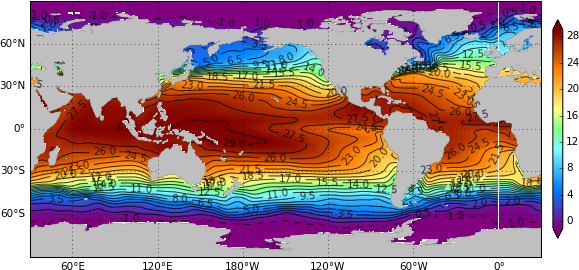
\includegraphics[scale=0.6]{./figures/woa09_temperature_0_annual.png}
  \end{center}
\end{frame}


\begin{frame}
\frametitle{Distribuição temperatura em 1000 m}
  \begin{center}
    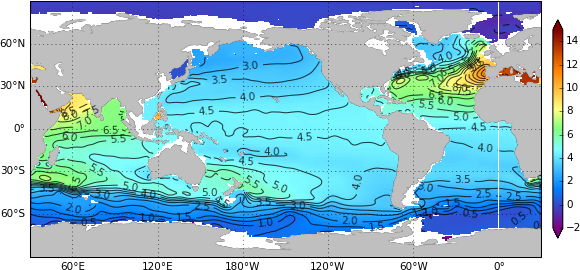
\includegraphics[scale=0.6]{./figures/woa09_temperature_1000_annual.png}
  \end{center}
\end{frame}


\begin{frame}
\frametitle{Distribuição temperatura em 4500 m}
  \begin{center}
    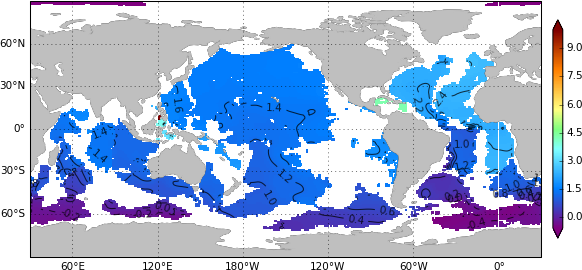
\includegraphics[scale=0.6]{./figures/woa09_temperature_4500_annual.png}
  \end{center}
\end{frame}


\begin{frame}
\frametitle{Distribuição temperatura (verão austral)}
  \begin{center}
    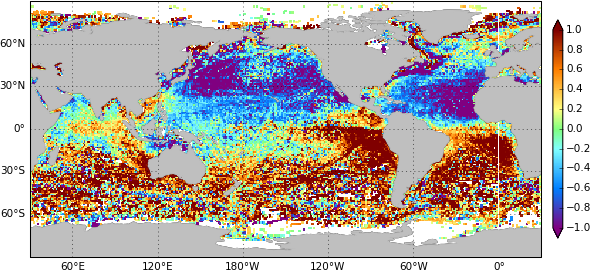
\includegraphics[scale=0.6]{./figures/woa09_temperature_summer_anomaly.png}
  \end{center}
\end{frame}


\begin{frame}
  \frametitle{Distribuição horizontais salinidade}
  \small{
  \begin{itemize}[<+-| alert@+>]
    \item Assim como a temperatura a distribuição da salinidade na superfície
          do oceano é aproximadamente zonal;
    \item Os mínimos estão próximos das altas latitudes e próximo ao
          continente;
    \item Os máximos se encontram nas regiões dos ventos alísios.
    \item Os fatores que levam a variações de salinidade são
          evaporação/precipitação e congelamento/degelo.
    \item Os mares Vermelho e Mediterrâneo têm salinidades de 39 e 41
          respectivamente.
  \end{itemize}
  }
\end{frame}


\begin{frame}
\frametitle{Distribuição salinidade}
  \begin{center}
    \includegraphics[scale=0.35]{../figures/evaporation_precipitaion.png}
  \end{center}
\end{frame}


\begin{frame}
\frametitle{Distribuição salinidade na superfície}
  \begin{center}
    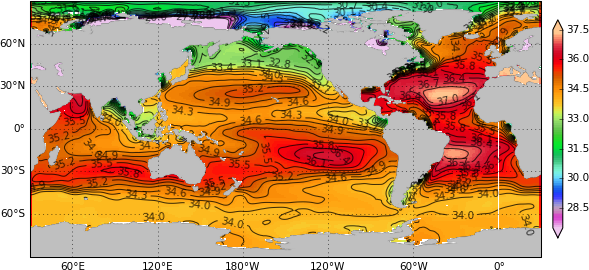
\includegraphics[scale=0.6]{./figures/woa09_salinity_0_annual.png}
  \end{center}
\end{frame}


\begin{frame}
\frametitle{Distribuição salinidade em 1000 m}
  \begin{center}
    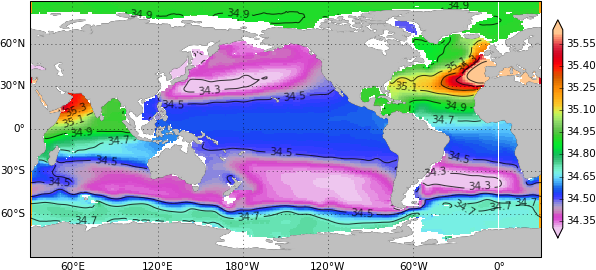
\includegraphics[scale=0.6]{./figures/woa09_salinity_1000_annual.png}
  \end{center}
\end{frame}


\begin{frame}
\frametitle{Distribuição salinidade em 4500 m}
  \begin{center}
    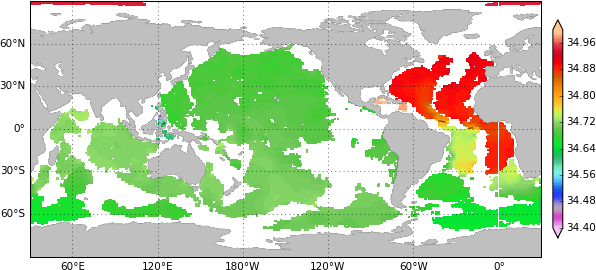
\includegraphics[scale=0.6]{./figures/woa09_salinity_4500_annual.png}
  \end{center}
\end{frame}


\begin{frame}
\frametitle{Distribuição salinidade (verão austral)}
  \begin{center}
    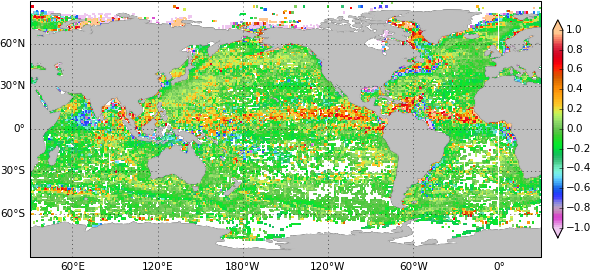
\includegraphics[scale=0.6]{./figures/woa09_salinity_summer_anomaly.png}
  \end{center}
\end{frame}


\begin{frame}
\frametitle{Distribuição salinidade}
  \begin{center}
    \includegraphics[scale=0.25]{../figures/annual_surface_salinity_with_ep.png}
  \end{center}
\end{frame}


\section{Distribuição vertical}
\begin{frame}
\frametitle{Plataforma continental X oceano profundo}

  \begin{center}
    \includegraphics[scale=0.4]{../figures/continental_plataform.png}
  \end{center}

  \begin{block}{}
  \scriptsize{
    PC: Declives 1:500 metros e largura entre 5--200 km;

    Quebra da plataforma: 50 a 200 m;

    TC: Declives 1:20 metros e largura entre 20--100 km.
    }
  \end{block}
\end{frame}


\begin{frame}
  \frametitle{Distribuição vertical de temperatura}
  \small{
  \begin{itemize}[<+-| alert@+>]
    \item Entre aproximadamente 200--300 m e 1.000 m de profundidade, a
          temperatura decresce rapidamente ``termoclina permanente'';
    \item Abaixo dessa região, em torno de 1.000 m de profundidade não existe
          variação sazonal e (exceto em regiões polares);
    \item $<$ 1.000 m a temperatura decresce suavemente entre 0\textcelsius{} e
          3\textcelsius{}.
    \item Essa faixa limitada é mantida em todo o oceano profundo,
          geograficamente e sazonalmente, pois é determinada pela temperatura
          de resfriamento e pela água densa que mergulha das regiões polares
          para o fundo do oceano em direção ao Equador.
  \end{itemize}
  }
\end{frame}


\begin{frame}
  \frametitle{Termoclina: Sazonal e diária}
  \scriptsize{
  \begin{itemize}[<+-| alert@+>]
    \item No inverno a temperatura na superfície baixa, as ondas são grandes
          e a camada de mistura é profunda podendo estender-se até à
          termoclina permanente.  No verão a temperatura da superfície aumenta,
          a água é mais estável e desenvolve-se uma Termoclina Sazonal.
    \item Em altas latitudes a temperatura na superfície é baixa assim como a
          temperatura das águas profundas.  Em consequência a termoclina
          permanente não existe, desenvolvendo-se apenas uma termoclina
          sazonal.
    \item Termoclinas Diurnas podem formar-se em qualquer local, desde que
          haja um suficiente aquecimento da superfície durante o dia.
    \item Elas ocorrem até profundidades de apenas 10--15 m e as diferenças de
          temperatura através delas não ultrapassam normalmente os 12\textcelsius{}.
  \end{itemize}
  }
\end{frame}


\begin{frame}
  \frametitle{Distribuição vertical de salinidade}
  \small{
  \begin{itemize}[<+-| alert@+>]
    \item Na superfície são encontradas as maiores variações de salinidade;
    \item Logo abaixo da camada de mistura temos a haloclina, ou região de
          maior gradiente de salinidade;
    \item Observa-se um mínimo permanente entre 600 e 1.000 m;
    \item Em região $>$2.000 m a salinidade volta a aumentar.
    \item Nos trópicos é comum um máximo de salinidade a cerca de 100 m.
    \item Nas altas latitudes, onde o valor à superfície é baixo, a salinidade
          em geral cresce com a profundidade até cerca de 2.000 m, sem o mínimo
          subsuperficial.
  \end{itemize}
  }
\end{frame}


\begin{frame}
\frametitle{Distribuição na coluna d'água}
  \begin{center}
    \includegraphics[scale=0.3]{../figures/coastal_profiles.png}
  \end{center}
\end{frame}


\begin{frame}
\frametitle{Distribuição na coluna d'água}
  \begin{center}
    \includegraphics[scale=1.6]{../figures/deep_vertical_profiles.png}
  \end{center}
\end{frame}


\begin{frame}
\frametitle{Perfis verticais médios típicos de salinidade nos oceanos}
  \begin{center}
    \includegraphics[scale=0.35]{../figures/vertical_profile_salinity_oceans.png}
  \end{center}
\end{frame}


\begin{frame}
\frametitle{Perfis verticais médios típicos de salinidade nos oceanos}
  \begin{center}
    \includegraphics[scale=0.35]{../figures/vertical_profile_temperature_oceans.png}
  \end{center}
\end{frame}


\begin{frame}
\frametitle{Termoclina}
  \begin{center}
    \includegraphics[scale=0.3]{../figures/termoclina.png}
  \end{center}
  \scriptsize{Obs: Qual seria a distribuição vertical de temperatura em
                   equilíbrio? O que e equilíbrio?}
\end{frame}


\section{Distribuição meridional}
\begin{frame}
\frametitle{Distribuição meridional de temperatura}
  \begin{center}
    \includegraphics[scale=0.35]{../figures/meridional_temperature.png}
  \end{center}
\end{frame}

\begin{frame}
\frametitle{Distribuição meridional de salinidade}
  \begin{center}
    \includegraphics[scale=0.35]{../figures/meridional_salinity.png}
  \end{center}
\end{frame}


\begin{frame}
\frametitle{Distribuição de densidade}
  \begin{center}
    \includegraphics[scale=0.65]{../figures/meridional_sigma.png}
  \end{center}
  \pause
  \small{Obs: Veremos isso com mais detalhe em breve!}
\end{frame}


\begin{frame}
\frametitle{Distribuição de massas d'água}
  \begin{center}
    \includegraphics[scale=0.25]{../figures/meridional_watermasses.png}
  \end{center}
  \pause
  \small{Obs: Veremos isso com mais detalhe em breve!}
\end{frame}


\section{Considerações finais}
\begin{frame}
  \frametitle{Considerações finais -- Importâncias}
  \scriptsize{O oceano afeta o tempo e os climas de muitas maneiras:
  \begin{itemize}[<+-| alert@+>]
    \item Correntes oceânicas quentes advectam calor para os polos para
          compensar o ganho de radiação líquida em baixas latitudes e o déficit
          em altas latitudes;
    \item TSM próximo à costa influenciam temperaturas do ar no litoral, a
          nebulosidade e a precipitação;
    \item A diferença entre as temperaturas do ar no litoral durante o dia e a
          TSM costeira induz brisas marítimas;
    \item A uniformidade dos oceanos, comparada com a superfície acidentada da
          terra, permite ventos mais fortes no mar e nas costas.
    \item As anomalias de TSM de oceanos próximos ou remotos afetam as chuvas e
          as secas;
    \item  A evaporação dos oceanos é a fonte principal de umidade de umidade
           atmosférica e é governada pela TSM;
    \item  Grandes áreas de oceanos frios ao longo das costas oeste e subtropicais frequentemente criam nuvens stratus, principalmente no verão e algumas podem se
deslocar para o litoral como nevoeiro advectivo;
    \item  Águas costeiras frias reduzem a chuva.
    \end{itemize}
    }
\end{frame}


\end{document}
